	\section{Hemorrhagic shock: a lethal but preventable condition}
	\label{shock}
		\subsection{Description}
Post-traumatic bleeding is the primary cause of preventable deaths among injured patients around the world \cite{WHO}\cite{urban}. When a person sustains a severe injury (e.g. due to a car accident or violent assault), she may present serious internal or external bleeding. If the injury is serious enough, the natural coagulation process is not sufficient to stop the blood loss. In that case, if too much blood is lost, the patient enters a state called hemorrhagic shock (HS) where the body is no longer able to provide vital organs with enough dioxygen to sustain them \cite{HS_def}. At this point, even proper care may not be enough to save the patient \cite{dutton2007current}.

When an individual sustains an injury, she is usually first taken in charge by first responders who evaluate the situation and the patient's state, before transporting her to a trauma centre when the patient will be treated.
To prevent patients from falling into HS, procedures have been established in most hospitals to trigger a fast response to suspected haemorhhage \cite{pommerening2015gestalt}: massive transfusion (MT) protocols can be activated even before the patient enters the hospital \cite{malone2006MT}. When this happens, the hospital gets ready to transfuse the patient with large amounts of blood as soon as she arrives, and frees up the necessary personnel. This way, the time interval between the injury and the transfusion in minimal. Studies \cite{hoyt1994death} \cite{martin2009combatSupport} show that early transfusion, followed by surgical bleeding control if necessary, can greatly improve the survival odds of patients that are at risk of entering hemorrhagic shock.

This means that it is essential to activate the procedure as early as possible if a patient's condition requires it. Unfortunately, it is quite hard to evaluate whether a patient is at risk of hemorrhagic shock\cite{pommerening2015gestalt}. While external bleeding (e.g. from a knife wound) is obvious, internal bleeding (usually from blunt trauma) on the other hand is not easily diagnosed visually or using physiological parameters (heart rate, blood pressure, \ldots) \cite{frank2010bloodLoss}. A full-body scan or at least an ultrasound examination may be needed\cite{perera2010rush}. This results in a significant delay in the activation of the procedure.

		\subsection{Motivation for an assistance tool}
%Prediction is very hard, as described in \cite{doctors_prediction} + possible to treat if taken early

As we mentioned, it is both far from obvious and very important to diagnose a risk of HS early, and doctors often fail to do so without advanced tests: a study \cite{pommerening2015gestalt} showed doctors to have quite limited performance when trying to predict a patient's risk of HS even after 10 minutes in the hospital. This highlights the difficulty of evaluating the need for the MT procedure before arrival, even when a doctor is present in the ambulance.

This combination of factors means that it makes sense to try to provide tools that would assist a doctor in detecting possible HS. To that end, a number of scoring systems have been developed to evaluate the risk of HS for a patient \cite{nunez2009ABC} \cite{gonzalez2016resussitation_outcome} \cite{maegele2011TASH}: the idea is to determine a set of conditions on physiological measurements that determine a numeric score for the patient. The idea is that with well-chosen criteria, the score gives an objective assessment of a patient's condition that can supplement a doctor's expertise, or be used directly as a prediction (e.g. if the score is higher than some threshold, then the patient is at risk). However, the same study that evaluated the performance of doctors' prediction \cite{pommerening2015gestalt} showed that numeric criteria perform no better than doctors in predicting HS.

This might mean that it is simply impossible to accurately predict HS before advanced examinations are performed. However, it is also possible, that the relations between HS and physiological measurements are complex enough that a simple hand-made criterion is not enough to capture them. In that case, it would be useful to build a statistical model capable of representing this relationship and of providing hospitals with early estimates of a patient's level of risk. 

This is why a team of researchers is trying to develop a tool that would leverage machine learning techniques to predict hemorrhagic shock, using a database of patient records (cf Section \ref{traumabase}). Our paper is part of that effort, with a specific focus on missing data imputation.

	\section{The Traumabase data}
	\label{traumabase}
		\subsection{The Traumabase project}
	
		\subsection{Data overview}
		
			\subsubsection{General information}
The Traumabase contained the records of 7477 patients at the time of this work. On recommendation of the doctors we worked with, we removed patients who sustained penetrating injuries such as knife or gunshot wounds --- 826 patients --- (because the presence of a hemorrhage is obvious to assess in this case) and those who had a cardiac arrest before their arrival in the hospital --- 396 patients --- because this level of gravity is always enough to justify an emergency procedure. We also excluded patients who were redirected to the trauma centre from another hospital (as opposed to directly by the first responders) --- 1102 patients --- since this does not correspond to our case of study (prehospital evaluation). This leaves us with a total of 5153 patients.

In this population, 500 patients went through hemorrhagic shock and 4653 did not.
			
The Traumabase records dozens of variables that trace a patient's history from the moment first responders arrive to the end of the patient's stay in the hospital (i.e. death or recovery). Here we are interested in performing a prehospital evaluation, so when we perform the prediciton we only consider a few measurements that correspond to those performed by the first responders. 

			\subsubsection{Definition of the variables}
There are 9 variables in the data that we can use for prediction.
\paragraph{General physical criteria}
These values are the sex, age and BMI (body-mass index) of the patient. They do not give any direct indication of shock, but they are necessary to control for natural differences between individuals (for instance, males naturally have a higher level of hemoglobin in their blood than females).

\paragraph{Basic physiological measurements}
These values are measured by the response team as soon as they arrive at the scene. They are:
\begin{enumerate}
\item Heart rate: The heart rate of the patient. Intuitively, if the patient has been losing blood, their heart should be beating faster in order to keep supplying the body with oxygen in spite of  the blood loss \cite{gutierrez2004clinical}
\item Pulse pressure: The difference between the systolic (maximal) and diastolic (minimal) blood pressure during a heart beat. When the volume of blood is the body is low, this pressure may decrease \cite{gutierrez2004clinical}
\item Hemoglobin level: This is the concentration of hemoglobin (Hb) in the blood. The blood is composed, among other things, of red blood cells which contain hemoglobin that is used to carry oxygen. During blood loss, the liquid part of the blood can be regenerated faster than the red cells \cite{gutierrez2004clinical} which causes a drop in the Hb concentration. It is easily measured on location using measurement kits \cite{lamhaut2011hemocue}.
\item Peripheral oxygen saturation: This value ranges from 0\% to 100\% and represents the fraction of Hb molecules in the blood carrying dioxygen. During bleeding, if the oxygen carrying capacity is reduced (lower Hb concentration, lower blood flow due to hypotension, \ldots) then organs will draw more oxygen  relative to the total carrying capacity and the saturation will decrease \cite{cohn2007saturation}. Measurement is easy and standard \cite{rall1999oxymetry}.
\end{enumerate}

\paragraph{Glasgow coma scale (GCS)}
The GCS is a score assessing the conscious state of the patient \cite{jones1979GCS}. It is computed from three criteria (eye movement, verbal response, motor functions) and ranges from 3 (deep coma or death) to 15 (fully awake). It gives a standardized way of reporting a patient's consciousness.

\paragraph{Volume expander injection}
To stabilise the patient and compensate major fluid loss, the emergency responder may decide to inject the patient with volume expanders \cite{kramer2003expander}, that is fluids specifically designed to fill some of the volume of the vascular system in order to rise blood pressure. This is a proxy for the responder's assessment of the patient's gravity, which is useful since many hard-to-quantify factors (paleness, gravity of the incident, general aspect, \ldots) may impact this assessment and would otherwise be unavailable to us.

This variable gives us the total volume (in mL) of expander that was injected into the patient.

			\subsubsection{Exploration}
\paragraph{Continuous variables:}
The following table gives a general summary of the continuous covariates:

\begin{tabular}{|c|c|c|c|c|}
\hline 
• & \textbf{Min} & \textbf{Max} & \textbf{Mean} & \textbf{Median} \\ 
\hline 
\textbf{Age} & 12 & 95 & 37.9 & 34 \\ 
\hline 
\textbf{BMI} & 12 & 100 & 24.8 & 24.2 \\ 
\hline 
\textbf{Heart rate} & 12 & 222 & 95.7 & 93 \\ 
\hline 
\textbf{Pulse pressure} & 0 & 169 & 46.3 & 45 \\ 
\hline 
\textbf{Hb level} & 0 & 19 & 13.9 & 14 \\ 
\hline 
\textbf{O2 saturation} & 0 & 100 & 96.5 & 98 \\ 
\hline 
\textbf{Expander} & 0 & 6250 & 791 & 500 \\ 
\hline 
\end{tabular} 

Their distribution is illustrated in Figure \ref{fig.eda_continuous}. We see that all the variables seem to have a unimodal distribution (some variables such as the expander are artificially rounded by the doctors when reporting, which accounts for the apparent drops in density). Additionally, an all variables but the expander dose, the mean and median are very close together.

The age has a rather heavy tail on the right (many old patients). The O2 saturation has a very long lower tail: while almost all patients are above 90\% saturation, it is much lower for a few patients. 

The differences between the populations of patients with and without shock are in line with our expectations: shocked patients have in general lower Hb levels, a higher heart rate, lower pressure and lower saturation. However, we also see that no single factor gives an easy separation, and that shocked patients can have normal readings for any given measurement.

\begin{figure}[h]
	\centering
   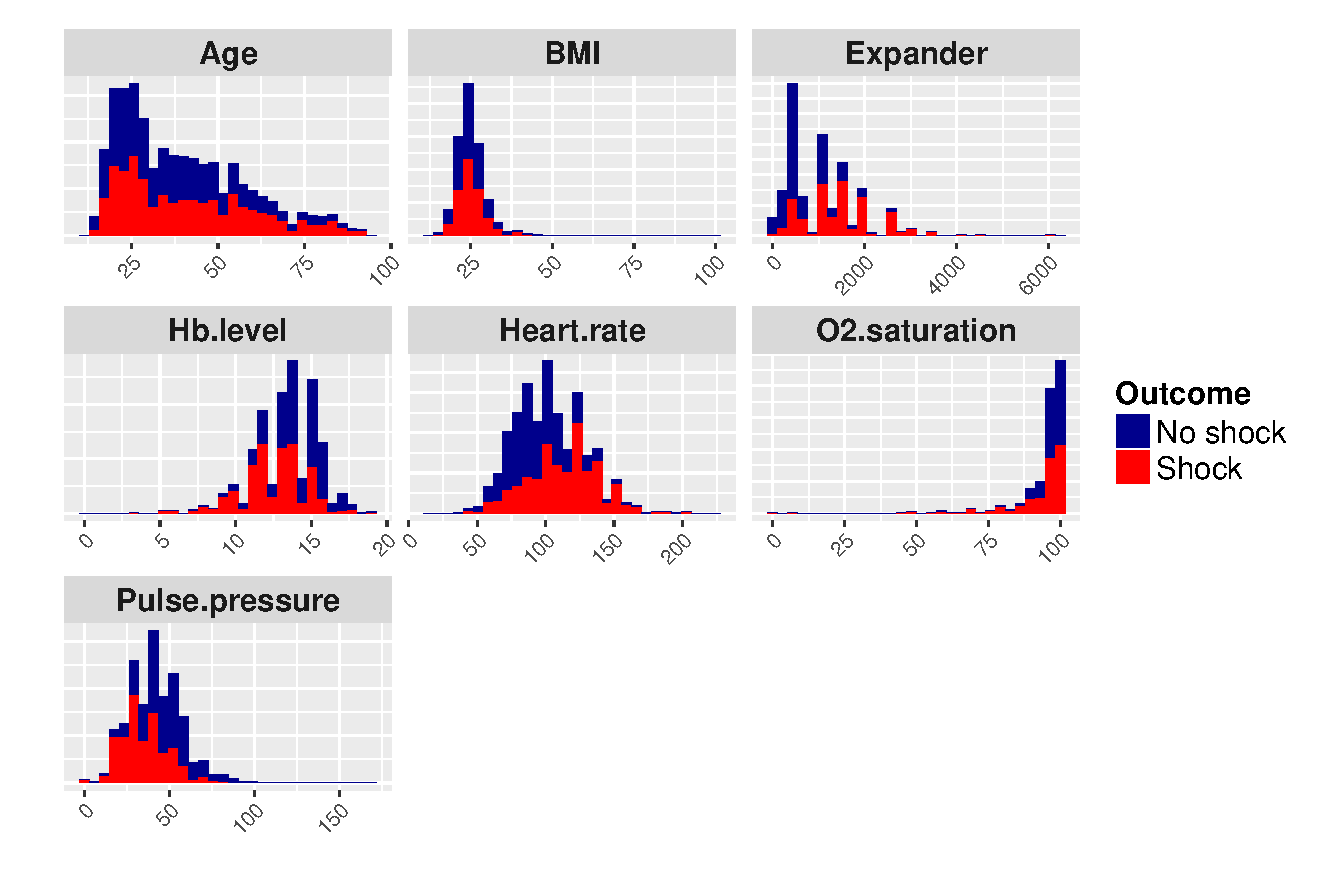
\includegraphics[scale=0.7]{Resources/eda_continuous}
   \caption{Distribution of the continuous variables depending on patient outcome}
   \label{fig.eda_continuous}
\end{figure}

\paragraph{Categorical variables}
We have just two variables which can be seen as categorical: the sex and the GCS score. For the GCS, this is a discrete scale from 3 to 15. Its distribution is shown on figure \ref{fig.eda_glasgow}. As before, shocked patients tend to have a lower score but many of them have a perfect score (15). 

As regards the sex, there are 1177 females and 3976 males in the population.

\begin{figure}[h]
	\centering
   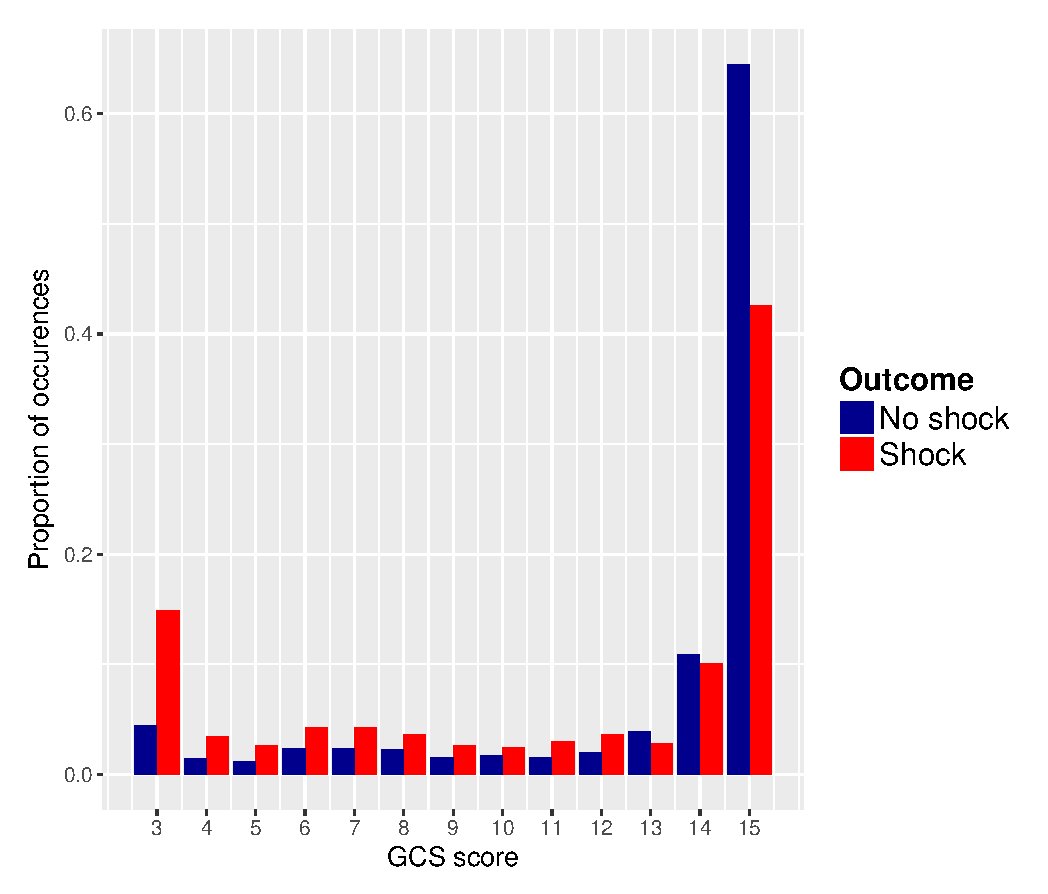
\includegraphics[scale=0.7]{Resources/eda_glasgow}
   \caption{Distribution of Glasgow Coma Scale score depending on patient outcome}
   \label{fig.eda_glasgow}
\end{figure}

\paragraph{Correlation structure}

Figure \ref{fig.cor_values} shows the correlation between the values of the observations (including the patient outcome). We see that not all variables have obvious correlation, but there are some subgroups of variables that are all correlated (e.g. Glasgow, heart rate, pulse pressure and saturation; or age, BMI and Hb level). 

As expected, the physical measurements (Sex, BMI, age) show no correlation with patient outcome, while all the other variables do. 

\begin{figure}[H]
	\centering
   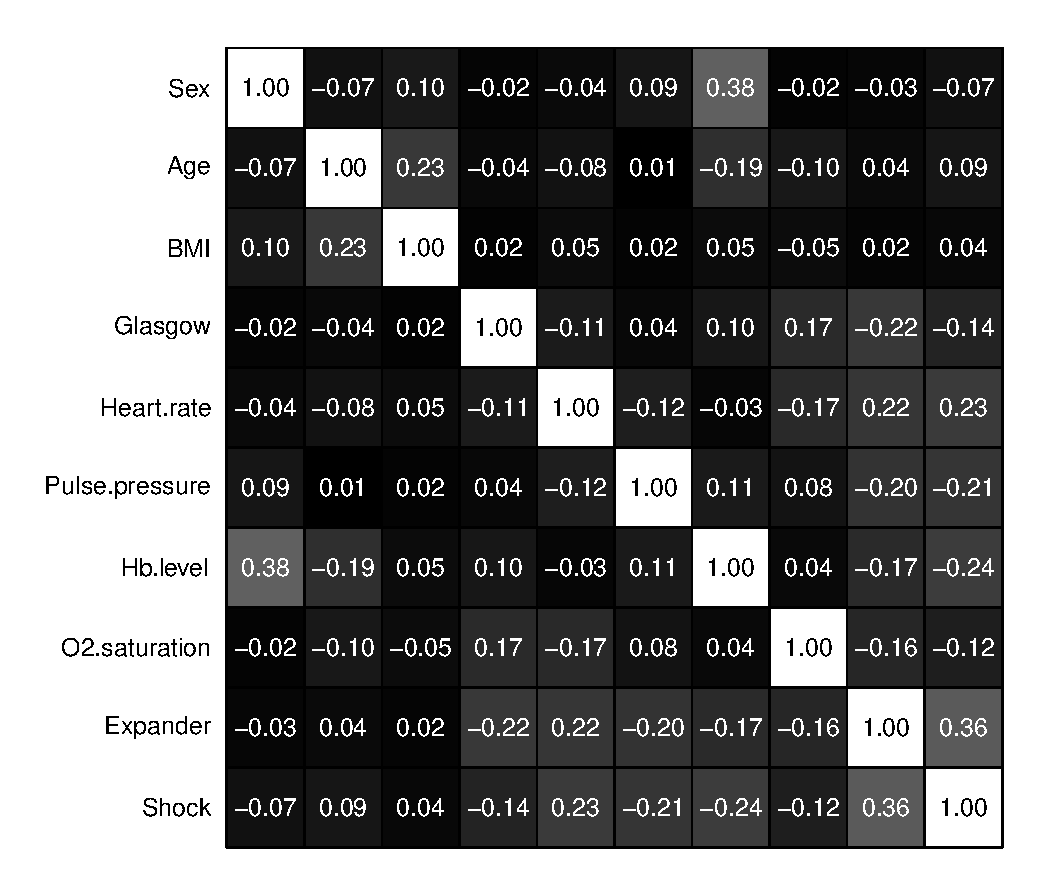
\includegraphics[scale=0.7]{Resources/cor_values}
   \caption{Correlation between the measurements (based on complete cases)}
   \label{fig.cor_values}
\end{figure}

			\subsubsection{Missing data}
			
An important aspect of the Traumabase is that is contains a significant amount of missing data. That is, some measurements or informations about the patients were not collected or not reported into the database, which makes them unavailable to us. In total, 5\% of the observations are missing. The table below gives the amount and proportion of missing data for each variable:

\begin{tabular}{|c|c|c|}
\hline 
• & \textbf{Amount} & \textbf{Proportion} \\ 
\hline
\textbf{Sex} & 0 & 0\% \\
\hline 
\textbf{Age} & 7 & 0.1\% \\
\hline 
\textbf{BMI} & 778 & 15\% \\ 
\hline
\textbf{GCS} & 18 & 0.4\% \\
\hline
\textbf{Heart rate} & 110 & 2.1\% \\ 
\hline 
\textbf{Pulse pressure} &  126 & 2.5\% \\ 
\hline 
\textbf{Hb level} &  301 & 5.8\% \\ 
\hline 
\textbf{O2 saturation} &  171 & 3.3\% \\ 
\hline 
\textbf{Expander} & 795 & 15.4\% \\ 
\hline 
\end{tabular} 

Figure \ref{fig.n_miss} shows the repartition of the number of missing observations in the data. 1686 patients (33 \%) have at least one missing observation.

\begin{figure}[h]
	\centering
   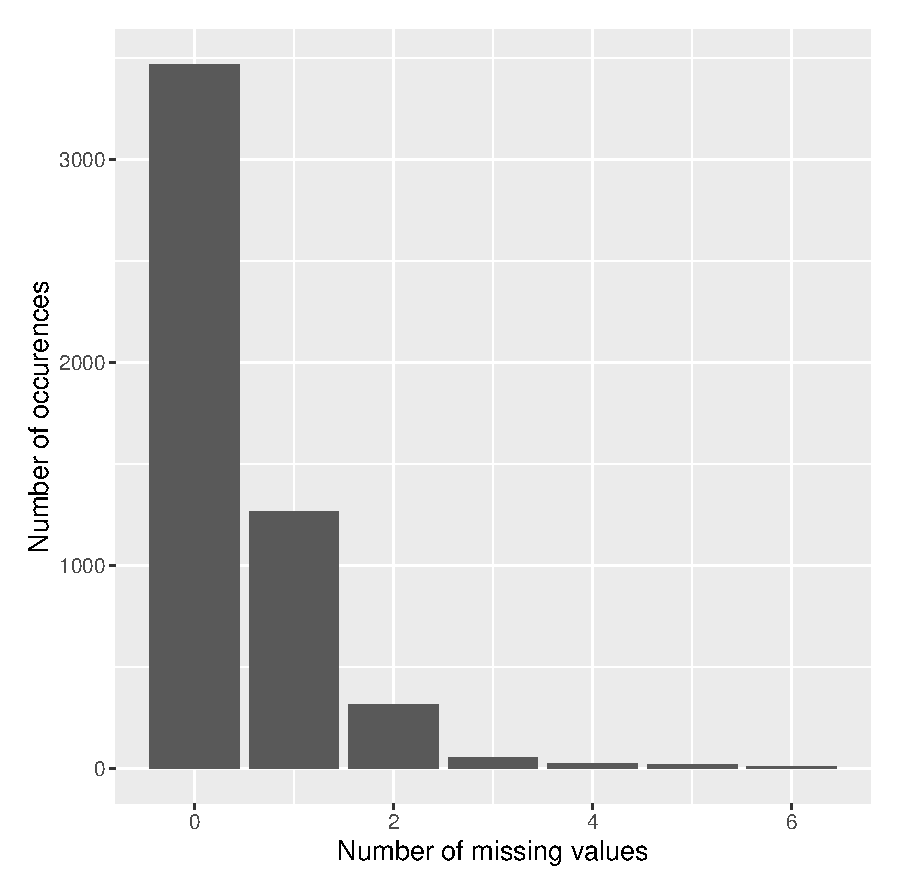
\includegraphics[scale=0.6]{Resources/n_miss}
   \caption{Distribution of the number of missing values per patient record}
   \label{fig.n_miss}
\end{figure}
			
Figure \ref{fig.cor_miss} shows the correlation between the missingness of the variables. They are mostly uncorrelated, but we see that physiological measurements tend to be missing at the same time.

\begin{figure}[H]
	\centering
   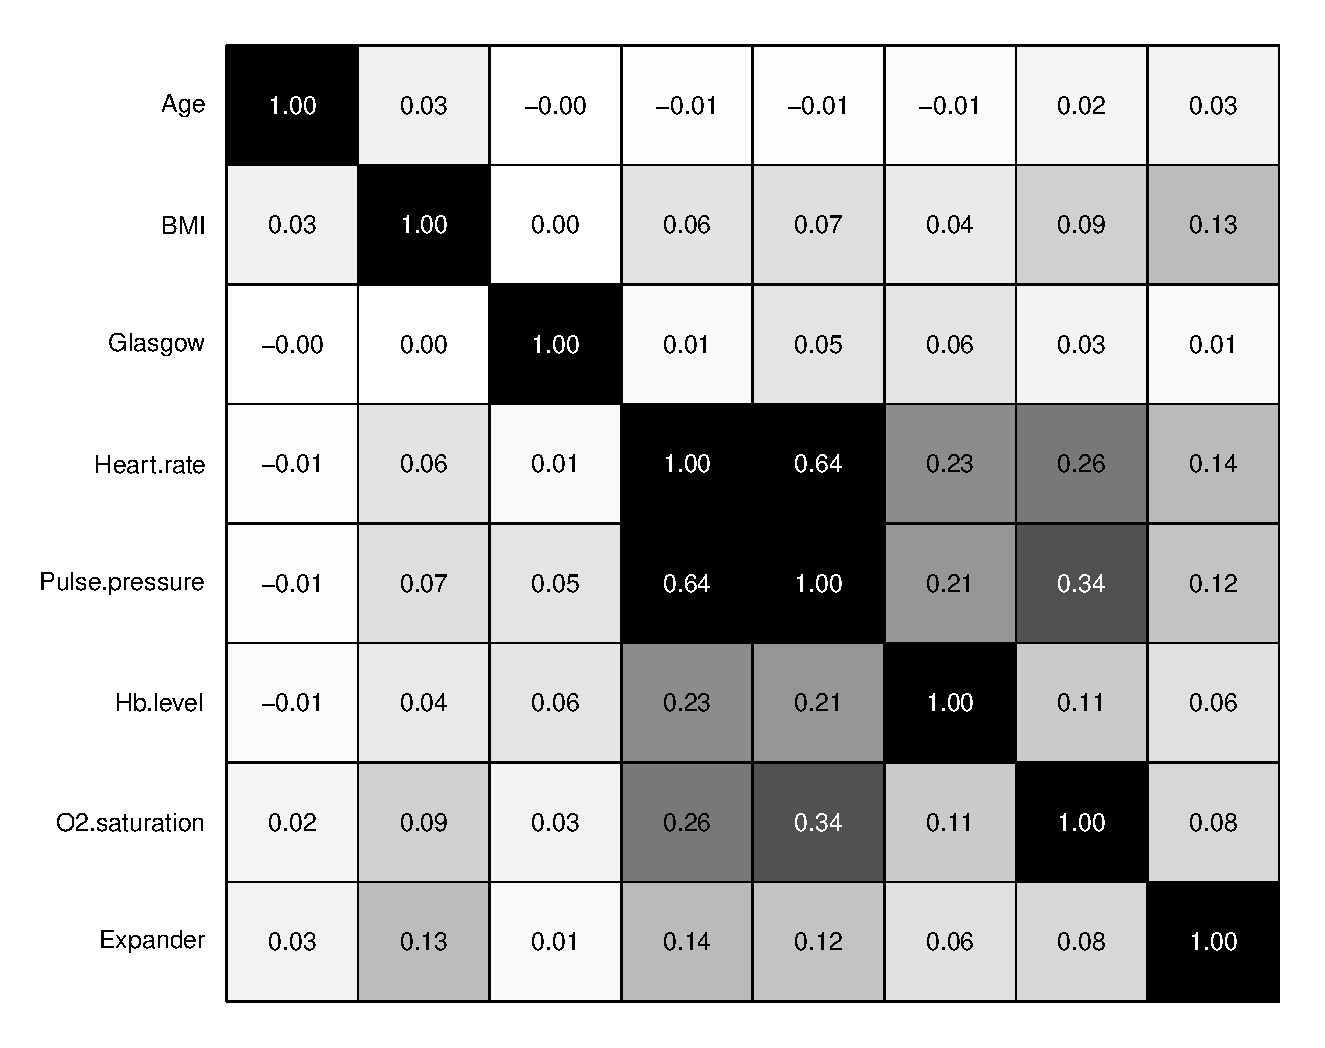
\includegraphics[scale=0.7]{Resources/cor_miss}
   \caption{Correlation between the missingness of each variable}
   \label{fig.cor_miss}
\end{figure}

Lastly, the table below gives the correlation between the missingness of each variable with the patient outcome:

\begin{tabular}{|c|c|}
\hline
\textbf{Age} & $5.7 \cdot 10^{-3}$\\
\hline 
\textbf{BMI} & $5.7 \cdot 10^{-3}$\\ 
\hline
\textbf{GCS} & $2.8 \cdot 10^{-3}$\\
\hline
\textbf{Heart rate} & $-7.6 \cdot 10^{-3}$  \\ 
\hline 
\textbf{Pulse pressure} &  $5 \cdot 10^{-2}$ \\ 
\hline 
\textbf{Hb level} &  $-4.5 \cdot 10^{-2}$ \\ 
\hline 
\textbf{O2 saturation} &  $0.11$ \\ 
\hline 
\textbf{Expander} & $-2.6 \cdot 10^{-2}$ \\
\hline 
\end{tabular} 

There is some amount of correlation between the missingness of the O2 saturation and the shock, but it is still quite low so it is hard to tell whether this has any significance.


	\section{Objective and formalization}
		\subsection{Objective of this work}
Given the importance of treating HS quickly, and the difficulty of detecting it --- especially for first responders not specialized in major trauma and do not have access to a hospital's equipment ---, there is a strong case for trying to predict HS automatically during the prehospital phase. This would enable a hospital to have an assessment of a patient's level of risk as soon as first responders reach them, and make preparations in advance to treat them urgently if necessary.
		
If one is to develop a tool that would predict hemorrhagic shock, an issue that will need to be addressed is that of missing data. Indeed, there are missing observations in the records of 33\% of the patients. Although this leaves us with a rather large number of complete cases, using only those would still be a major loss of information. Even more importantly, some data may also be missing in the real world when a prediction needs to be made. In that case, there no way around handling the missing observations to output a prediction.

In this work, we will address the particular issue of missing data, and more precisely of imputation: replacing the missing values in the dataset by plausible ones. Indeed, it is possible to create a model that takes missing data into account without trying to fill in the missing values and it has been done successfully in the past \cite{schafer2002missing}. However, existing missing-data implementations are fairly rare, so trying out any model means working almost from the ground up. This greatly limits our ability to compare several models.

Comparatively, once the dataset is imputed, it can be used with any existing complete-data prediction method. Additionally, it allows a separation of the tasks: the person or team performing the imputation is not necessarily the same as the one performing the subsequent analysis. Of course, this approach has drawbacks as well. In particular, once the dataset is imputed, any method used to perform a prediction with this dataset will use the observed and imputed values indiscriminately, which may lead to errors if the imputation is not correct.

 In the following chapters, we investigate the possibility of performing imputation in a predictive context, and how it should be done. Below we present the formal setting of the problem we investigate.
 
		\subsection{The God/Imputer/Analyst/Practitioner framework}
		\label{framework}
Let us recall the tasks at hand: imputing the data in the Traumabase, then applying a complete-data procedure to learn a model for the outcome. Finally, for new  incoming patients, use the new measurements (possibly with missing data) to evaluate whether they are at risk of HS. 

It is clear that form the point of view of the end user (the hospital or medical practitioner), the performance of this procedure should be judged by its predictive performance on new patients. This separation between historical data and new patients is central to our problem, and we investigate it further in chapters \ref{validation} and \ref{linreg}.

To formalize this setting, we draw inspiration from the framework proposed by Xie and Meng \cite{xie2017framework} to explore the issue of imputation. In their work, three actors come into play, God, the Imputer and the Analyst. We adapt this framework by adding a fourth actor, the Practitioner, who represents the end user who is only interested in prediction. Their interaction goes as follows:
\begin{itemize}
 \item "God" (i.e. nature) generates some data $\tilde{X}$ and outcome $y$ based on a process known only to him. 
 \item A dataset $X$ is generated by adding missing values to $\tilde{X}$. $X$ and $y$ are transferred to an Imputer. The Imputer is tasked with filling in the missing observations. She chooses an imputation model with parameter $\alpha$ and computes an estimate $\hat{\alpha}$ which she uses to generate a completed dataset $X_{imp}$.
 \item  The Imputer transfers $X_{imp}$ to an Analyst, along with $y$. The Analyst does not know which observations were initially missing.
 \item The Analyst uses $X_{imp}$ and $y$ to learn a predictive model with parameter $\beta$. Her estimation for this parameter is $\hat{\beta}$
 \item God generates a new pair of data and outcome $\tilde{X}_{new}, y_{new}$. Some missing data are added to  $\tilde{X}_{new}$ to generate $X_{new}$.
 \item The Practitioner receives $X_{new}$. She has no access to the data used for training. The Analyst and Imputer provide the Practitioner with black-box functions that allow her to perform imputation and prediction on the new data. They are derived from their model and parameter estimate; we call them $f(\cdot,\hat{\alpha}),g(\cdot,\hat{\beta})$.
 \item The Practitioner uses those functions to compute $X_{new}^{imp} = g(X_{new},\hat{\alpha})$ and $\hat{y}_{new}= f(X_{new}^{imp},\hat{\beta})$.
 \item $\hat{y}_{new}$ is finally compared to $y_{new}$ and the loss $L(y_V, \hat{y}_V)$ is computed. This gives the final performance evaluation of the process.
\end{itemize}

This process is illustrated in Figure \ref{fig.tikz_imp}

\begin{figure}[H]
  \includestandalone[width=\textwidth]{Charts/imputation_flowchart}%     without .tex extension
  \caption{Imputation framework}
  \label{fig.tikz_imp}
\end{figure}

The purpose of this formalization is to clarify the separation between the different phases of the inference, and show how the information is divided. Note that the separation between the Imputer and the Analyst is artificial --- we choose it because we are interested in performing imputation separately --- while the distinction between the Practitioner and the Analyst is imposed by the problem we are trying to solve: during an intervention, the users need a black-box tool that takes in the available data and outputs a prediction more or less instantly. Even if they had access to the training data, it would be impractical to learn a model all over again every time a new patient comes up. Additionally, the data we are using to learn the model cannot be widely shared since it contains patient records, so the Practitioner will not have access to it.

In a setting where all three roles are regrouped, the sensible way to proceed would be to define a joint model on the full data (including the response) and use it to find the maximum likelihood estimator for the unknown outcomes. However, the segmentation of the roles makes it necessary for each agent to work with partial information. In the rest of this work, we investigate the implications of this division, both in terms of theory and of practical implementation.

In Chapter \ref{imputation}, we present an overview of methods used for imputation. Chapter \ref{validation} considers the practical difficulties encountered when trying to impute new data with a previously learned model. Chapter \ref{linreg} explores the asymmetry that exists between missing values present in the training set and in the new data. Then, Chapter \ref{analysis} goes back to the Traumabase data to explore the best way to perform imputation in this particular case and Chapter \ref{results} presents our final results and compares the performance to that of doctors and criteria-based scores.